\documentclass[]{nsm-thesis}
% options:
% [germanthesis] - Thesis is written in German
% [plainunnumbered] - Don't print numbers on plain pages
% [earlydraft] - Settings for quick draft printouts
% [watermark] - Print current time/date at bottom of each page
% [phdthesis] - switch to PhD thesis style
% [twoside] - double sided
% [cutmargins] - text body fills complete page

% Author name. Separate multiple authors with commas.

\usepackage{acro}
\usetikzlibrary{quotes,angles}
\usepackage{nicefrac}

\author{Karl Christian Lautenschläger}
\birthday{29. Juni 1998}
\birthplace{Magdeburg}

% Title of your thesis.
\title{Suitability of Modern Wi-Fi for Wireless-Infield-Communication of Agricultural Machines}

% Choose one of the following lines, changing the word "Computer Science" to match your degree program.
\thesistype{Diploma Thesis in Information Systems Engineering}\thesiscite{Diploma Thesis~(Diplomarbeit)}

\advisors{Christoph Sommer}
% List of advisors (without academic titles), separated by commas.

% List of referees (without academic titles), separated by commas.
\referees{Christoph Sommer, Burkhard Hensel}

\DeclareAcronym{FH}{
	short=FH,
	long=Forage Harvester,
}
\DeclareAcronym{TM}{
	short=TM,
	long=Transport Machine,
}
\DeclareAcronym{BCC}{
	short=BCC,
	long=binary convolutional coding,
}
\DeclareAcronym{LDPC}{
	short=LDPC,
	long=low-density parity-check,
}
\DeclareAcronym{FEC}{
	short=FEC,
	long=Forward Error Correction,
}
\DeclareAcronym{WPA}{
	short=WPA,
	long=Wi-Fi Protected Access,
}

\DeclareAcronym{DCF}{
	short=DCF,
	long=Distribution Coordination Function,
}
\DeclareAcronym{DIFS}{
	short=DIFS,
	long=Distributed Coordination Function Interframe Space,
}
\DeclareAcronym{SSID}{
	short=SSID,
	long=Service Set Identifier,
}
\DeclareAcronym{SIFS}{
	short=SIFS,
	long=Short Interframe Space,
}
\DeclareAcronym{ACK}{
	short=ACK,
	long=Acknowledgement,
}
\DeclareAcronym{NAV}{
	short=NAV,
	long=Network Allocation Vector,
}
\DeclareAcronym{PCF}{
	short=PCF,
	long=Point Coordination Function,
}
\DeclareAcronym{CSMACA}{
	short=CSMA/CA,
	long=Carrier Sense Multiple
	Access/Collision Avoidance,
}

\DeclareAcronym{IBSS}{
	short=IBSS,
	long=Independent Basic Service Set,
}
\DeclareAcronym{AP}{
	short=AP,
	long=Access Point,
}
\DeclareAcronym{PPD}{
	short=PPD,
	long=Plant Population Density,
}
\DeclareAcronym{WIC}{
	short=WIC,
	long=Wireless-Infield Communication,
}
\DeclareAcronym{M2M}{
	short=M2M,
	long=Machine-To-Machine,
}

\DeclareAcronym{MIMO}{
	short=MIMO,
	long=Multiple Input Multiple Output,
}
\DeclareAcronym{STBC}{
	short=STBC,
	long=Space-Time-Block-Code,
}
\DeclareAcronym{PPDU}{
	short=PPDU,
	long=Physical layer convergence protocol data unit,
}
\DeclareAcronym{MCS}{
	short=MCS,
	long=Modulation
	and Coding Scheme,
}
\DeclareAcronym{CR}{
	short=CR,
	long=Coding Rate,
}
\DeclareAcronym{GI}{
	short=GI,
	long=Guard Interval,
}
\DeclareAcronym{DCM}{
	short=DCM,
	long=Dual Carrier Modulation,
}
\DeclareAcronym{MANET}{
	short=MANET,
	long=Mobile Ad Hoc Network
	and Coding Scheme,
}  

\DeclareAcronym{ASC}{
	short=ASC,
	long=Automatic Section Control,
}
\DeclareAcronym{m-ASC}{
	short=m-ASC,
	long=Meshed Automatic Section Control,
}
\DeclareAcronym{AEF}{
	short=AEF,
	long=Agricultural Industry Electronics Foundation,
}
\DeclareAcronym{FMIS}{
	short=FMIS,
	long=Farm Management Information System,
}
\DeclareAcronym{hTMM}{
	short=hTMM,
	long=Hybrid Threat Modeling Method,
}
\DeclareAcronym{STRIDE}{
	short=STRIDE,
	long= Spoofing\, Tampering\, Repudiation\, Information disclosure\, Denial of services\, and Escalation
	of privileges,
}
\DeclareAcronym{PASTA}{
	short=PASTA,
	long= Process for Attack Simulation and Threat Analysis,
}

\DeclareAcronym{ac}{
	short=802.11ac,
	long= IEEE 802.11ac,
}

\DeclareAcronym{ax}{
	short=802.11ax,
	long= IEEE 802.11ax,
}

\DeclareAcronym{OFDMA}{
	short=OFDMA,
	long= Orthogonal Frequency-Division Multiple Access,
}
\DeclareAcronym{OFDM}{
	short=OFDM,
	long= Orthogonal Frequency-Division Multiplexing,
}
\DeclareAcronym{RU}{
	short=RU,
	long= Resource Unit,
}
\DeclareAcronym{SINR}{
	short=SINR,
	long= Signal-to-Interference-plus-Noise Ratio,
}
\DeclareAcronym{QAM}{
	short=QAM,
	long=Quadrature Amplitude Modulation,
}
\DeclareAcronym{PSK}{
	short=PSK,
	long=Phase Shift Keying,
}
\DeclareAcronym{RSS}{
	short=RSS,
	long=Received Signal Strength,
}
\DeclareAcronym{SNR}{
	short=SNR,
	long=Signal Noise Ratio,
}
\DeclareAcronym{PDR}{
	short=PDR,
	long=Packet Delivery Ratio,
}
\DeclareAcronym{LOS}{
	short=LOS,
	long=Line-of-sight,
}
\DeclareAcronym{ESS}{
	short=ESS,
	long=Extended Service Set,
}
\DeclareAcronym{BSS}{
	short=BSS,
	long=Basic Service Set,
}
\DeclareAcronym{V2X}{
	short=V2X,
	long=Vehicle-to-everything,
}


% Define abbreviations used in the thesis here.
\acrodef{WSN}{Wireless Sensor Network}

\acrodef{ROI}{Region of Interest}{short-indefinite={an}, long-plural-form={Regions of Interest}}
\acrodef{ADAC}{German Automobile Association}{foreign={Allgemeiner Deutscher Automobilclub}}
\acrodef{CANhashing}[CAN]{Content Addressable Network}{extra={when referring to the distributed hash table}}
\acrodef{CANproto}[CAN]{Controller Area Network}{extra={when referring to the bus protocol}}

\begin{document}

\pagenumbering{roman}

\maketitle

\cleardoublepage

\TODO{This template is for use with \texttt{pdflatex} and \texttt{biber}. It has been tested with TeX~Live 2020 (as of 25 Oct 2020).}

\chapter*{Abstract}
\addcontentsline{toc}{chapter}{Abstract}
\begin{otherlanguage*}{american}

about 1/2 page:
\begin{enumerate}
    \item Motivation (Why do we care?)
    \item Problem statement (What problem are we trying to solve?)
    \item Approach (How did we go about it)
    \item Results (What's the answer?)
    \item Conclusion (What are the implications of the answer?)
\end{enumerate}

The abstract is a miniature version of the thesis.
It should be treated as an entirely separate document.
Do not assume that a reader who has access to an abstract will also have access to the thesis.
Do not assume that a reader who reads the thesis has read the abstract.

\end{otherlanguage*}


\chapter*{Kurzfassung}
\addcontentsline{toc}{chapter}{Kurzfassung}
\begin{otherlanguage*}{ngerman}

Gleicher Text (sinngemäß, nicht wörtlich) in Deutsch

\end{otherlanguage*}
\acresetall

\cleardoublepage
\tableofcontents
\TODO{The table of contents should fit on one page. When in doubt, adjust the \texttt{tocdepth} counter.}

\cleardoublepage
\pagenumbering{arabic}


\chapter{Introduction}
%\chapter{Einleitung}
\label{sec:introduction}

\begin{itemize}
\item general motivation for your work, context and goals.
\item context: make sure to link where your work fits in
\item problem: gap in knowledge, too expensive, too slow, a deficiency, superseded technology
\item strategy: the way you will address the problem
\item recommended length: 1-2 pages.
\end{itemize}




\chapter{Fundamentals}
\label{sec:fundamentals}



\begin{itemize}
\item describe methods and techniques that build the basis of your work
\item include what's needed to understand your work (e.g., techniques, protocols, models, hardware, software, ...)
\item exclude what's not (e.g., anything you yourself did, anything your reader can be expected to know, ...)
\item review related work(!)
\item recommended length: approximately one third of the thesis.
\end{itemize}

\TODO{
	-1/3 ist kurz, weil der Bezug und die Relation zur Landwirtschaft groß ist... Aber wen interessiert das? 
-1/3  related Work erwähnt man dann Unterstützung von Professor Klingler wie und wo? erwähnt man sich selber ?  
`}
\section{\acl{WIC}}

\todo[color=blue]{Den Teil haben mehrere Leute Korrektur gelesen. Den musst du nicht überfliegen, da man ihn kaum für das Verständnis braucht.}
Since 2014, the \ac{WIC} project group has been working on the development of a for \ac{WIC} standard, which covers a standard for machine-to-machine communication, encryption, and security \footnote{https://www.aef-online.org/about-us/teams.html}.
\textcite{schlingmann_aef_2019} summarize the goals of the \ac{WIC} project team as follows:
\begin{itemize}
	\item Define use cases for \ac{WIC} in agriculture
	\item Evaluate the suitability of communication technologies
	\item Find suitable communication protocols
	\item Standardize the \ac{WIC} common software library
	\item Develop functional and security requirements and concepts
	\item Test first prototypes in regards of cross-brand comformance
	\item Write a application guideline
\end{itemize}
First steps have already been taken in this direction. The use cases and key scenarios are defined and explained by the authors as follows:
\begin{itemize}
	\item \textbf{Real-Time Machine-to-Machine Control} is the exchange of control data under real-time conditions with defined latency policies. This use case enables leader-follower scenarios where agricultural machines follow a leading agricultural machine at a lateral and longitudinal distance. Throughout this thesis, I will refer to Real-Time Machine-to-Machine Control as Agricultural Platooning Service.
	%\TODO{Fendt-Paper? Auch erwähnen eigentlich ja später, Beispiel aus AEF Paper?}
	\item \textbf{Streaming Services} are communications that stream video from remote cameras and monitors at a high data rate and low latency. The authors estimate the distance between the communication participants to be less than \SI{100}{\metre}. As a result, this data is available on another agricultural vehicle and can be analyzed and processed there.
	I will refer to Streaming Services as Agricultural Streaming Services in this thesis. %\TODO{Camera harvest streaming}
	\item \textbf{Process Data Exchange} describes the exchange of process data. One example is the exchange of already sprayed field areas to prevent multiple spraying of fertilizers and pesticides on the same field area by different machines. According to the authors, this \ac{WIC} use case requires long-range technologies because agricultural fields worldwide can be vast.
	%\TODO{ISO 11783-10 extended FMIS Data Interface}
	\item \textbf{Fleet Management \& Logistics} is the potential retrieval of data from the ongoing agricultural process. This information can influence economic or agronomic decisions of agricultural enterprises or service companies and is therefore required in a \ac{FMIS}.
	Since not all agricultural machines may be connected to the \ac{FMIS}, the \ac{WIC} project group is looking at how to use \ac{M2M} communications to bridge the missing communications infrastructure until the data reaches a machine that can connect to the \ac{FMIS}.
	\item \textbf{Road Safety} describes a use case which is already a project between the European Telecommunication Standard Institute and the \ac{AEF}. Since agricultural vehicles are repeatedly underestimated in their size and speed by other road users when they suddenly turn off the field onto the road, the other road users need to be warned in this situation. In this way, smart technologies in cars and motorcycles can brake these vehicles in advance and prevent possible accidents.
\end{itemize}

\todo[color=blue]{Wichtig:}
Considering that I investigate the Suitability of modern Wi-Fi for Wireless-Infield-Communication and modern Wi-Fi like IEEE 802.11ax is no long range technologies,
I will focus on investigating the suitability of IEEE 802.11ax for the \ac{WIC} use case Real-Time Machine-to-Machine Control.
Throughout this thesis, I will refer to real-time machine-to-machine control as Agricultural Platooning.
An example how farmers can benefit from Streaming Services or Agricultural Platooning Services is the corn harvesting and loading process.




\section{Wireless Lans according to IEEE 802.11}
\todo{Paper Christoph Sommer, Doktorarbeit, Diplomarbeit, Mario Franke, Tobias Hardes}
According to \textcite{kauffels_wireless_2002} the first version of the Standard IEEE 802.11 was published in 1999 to enable a wireless alternative to Ethernet - or Token-Ring - networks.
\textcite{sauter_wireless_2022} considers IEEE 802.11 also to be an implementation of Ethernet with the help of wirless radio technologies. The author lists the extensions to the original standard, which range from 802.11b, 802.11g, 802.11a, 802.11n, 802.11ac to the latest enhancement 802.11ax. The different IEEE 802.11 standards can operate in the  \SI{2.4}{\giga\hertz} - , \SI{5}{\giga\hertz} and \SI{6}{\giga\hertz} - frequency band. 
\textcite{jacobs} fügt dazu noch hinzu, dass es zusätzlich noch die zwei Erweiterungen IEEE 802.11p and dessen Nachfolger IEEE 802.11bd gibt. Diese operieren in einem reservierten Frequency spectrum for \ac{V2X} nach den Autoren im  \SI{5.9}{\giga\hertz} frequency spectrum
\todo{HT, VHT, HE - phy}

\textcite{kauffels_wireless_2002} defines the following three basic architectures for IEEE 802.11.

If two or more stations communicate directly without an AP, they form an ad hoc network. According to the author, this can be set up quickly and easily and is also called \ac{IBSS}.

The Infrastructure \ac{BSS} mode allows all stations within the range of defined range around the \ac{AP} to communicate via a central \ac{AP}. Within the area of the \ac{BSS}, all stations can move freely and communicate with one another.

Since an \ac{AP} has limited range and can only cover a certain area, the \ac{ESS} was introduced. It contains a distribution system, which links several \ac{BSS} with each other.

Thereby, the BSS coverage areas can physically overlap so that continuous connection of stations within the ESS can be provided. For a better performance the \ac{BSS} can be placed physically on top of each other. One can also have physically separate \ac{BSS}s so that these \ac{BSS}s can be linked together over long distances. According to the author, the standard does not specify a distance limit for such connections. 

He also mentions, that the standard defines the following three mobility types for station in an \ac{ESS}, where a station can do no-transition and thereby stay within a \ac{BSS}, \ac{BSS}-transitioning and move from one \ac{BSS} to another \ac{BSS} within the same \ac{ESS} and \ac{ESS}-transition, where the Station moves from a \ac{ESS} to another one but no stable connection can be guaranteed.

\textcite{sauter_wireless_2022} adds, that usually Ethernet is used to link \ac{AP}s in within an \ac{ESS}. But according to the author this can be replaced by a wireless connection, which is called wireless bridge.
\todo{ESS not needed?}

\TODO{Sauter 2022 Ad-Hoc Infos}
\subsection*{Wi-Fi Physical Layer}
A constant change of the physical layer accompanies the further development of IEEE 802.11.
\textcite{sauter_wireless_2022} mentions that all new enhancements of the physical layer of IEEE 802.11 are backward
compatible with previous definitions of the standard.

According to the Author, IEEE 802.11 initially used DSSS and FHSS as modulation methods.
Since IEEE 802.11g the modulation method \ac{OFDM} can be used in the \SI{2.4}{\giga\hertz} frequency band.
The author explains \ac{OFDM} as follows. \ac{OFDM} divides the transmission channel into subcarriers with different
amplitudes, frequencies and phases.
Each subcarrier is orthogonal to another one, as they send the information ``Low``,
where only one other subcarrier is sending the information ``High``.


\subsubsection*{Symbol length}
The data is then sent as \ac{OFDM} symbols over the individual \ac{OFDM} subcarriers.
The distance between the ``Highs`` of the subcarriers is specified as subcarrier spacing and corresponds to the reciprocal
symbol length.
IEEE 802.11ax increased the \ac{OFDM} symbol length from \SI{3.2}{\micro\second} for IEEE 802.11n to a maximum of \SI{12.8}{\micro\second} \cite{sauter_wireless_2022}.
This corresponds to a subcarrier spacing of \SI{312.5}{\kilo\hertz} and \SI{78.125}{\kilo\hertz} respectively \cite{sauter_wireless_2022}.

For the IEEE 802.11p and IEEE 802.11bd standards, a symbol length of \SI{6.4}{\micro\second} applies, corresponding to a subcarrier spacing of \SI{156.25}{\kilo\hertz} \cite{jacob_system-level_2020}.

The Fast Fourier Transform and Inverse Fast Fourier Transform are used to modulate and demodulate the transmitting bits.
With the reduction of subcarrier spacing, more subcarriers are created in the transmission channel,
so the Fast Fourier Transform size must be increased.

\textcite{kauffels_wireless_2002} adds that \ac{OFDM} can be used in the \SI{5}{\giga\hertz} frequency band since IEEE 802.11a.
\subsubsection*{\acf{BW}}
The frequency bands are divided into channels in order to create several transmission channels.
This results in 13 channels in Europe in the frequency band of \SIrange{2.412}{2.482}{\giga\hertz} and 18 channels in the frequency band of \SIrange{5.180}{5.350}{\giga\hertz} and \SIrange{5.180}{5.350}{\giga\hertz} \cite{sauter_wireless_2022}.
Transmission channels can be combined to enable higher data rates.
Every channel has a width called \ac{BW} specified in \si{\mega\hertz}.
The possible \ac{BW}s for the IEEE 802.11 standards are shown in \autoref{tab:BW}.
\begin{table}[!ht]
	\centering
	\begin{tabular}{>{\raggedright}p{2.2cm}p{2.50cm}p{2.55cm}p{2.50cm}}
		\toprule
		Standard & Channel \ac{BW}s\newline in \SI{2.4}{\giga\hertz}& Channel \ac{BW}s\newline in \SI{5}{\giga\hertz} &  Channel \ac{BW}s\newline in  \SI{5.9}{\giga\hertz}\\
		\midrule
		IEEE 802.11n \cite{sauter_wireless_2022}& \SI{20}{\mega\hertz},\SI{40}{\mega\hertz}  & \SI{20}{\mega\hertz},\SI{40}{\mega\hertz} & - \\
		\midrule
		IEEE 802.11ac \cite{noauthor_ieee_2021-1}& -  & \SI{20}{\mega\hertz},\SI{40}{\mega\hertz}, \SI{80}{\mega\hertz},\SI{160}{\mega\hertz} & - \\
		\midrule
		IEEE 802.11ax \cite{noauthor_ieee_2021}&\SI{20}{\mega\hertz},\SI{40}{\mega\hertz}  & \SI{20}{\mega\hertz},\SI{40}{\mega\hertz}, \SI{80}{\mega\hertz},\SI{160}{\mega\hertz} & - \\
		\midrule
		IEEE 802.11p \cite{jacob_system-level_2020}& - & - & \SI{10}{\mega\hertz} \\
		\midrule
		IEEE 802.11bd \cite{jacob_system-level_2020}& - & - & \SI{10}{\mega\hertz},\SI{20}{\mega\hertz} \\
		\bottomrule
	\end{tabular}
	\caption{Available \ac{BW}s for the IEEE 802.11 standards per frequency band.}
	\label{tab:BW}
\end{table}

IEEE 802.11ac and IEEE 802.11ax also enable the use of a discontinuous \ac{BW}, which combines two \SI{80}{\mega\hertz}
channel to a \SI{160}{\mega\hertz} \ac{BW} channel \cite{noauthor_ieee_2021}, \cite{noauthor_ieee_2021-1}.

While wider channels increase the theoretical data rate, \textcite{avallone_will_2021} mentions that narrower channels can
boost the signal's power spectral density and thus increase the transmission range.

\subsubsection*{\acf{MCS}}

In order to encode as many bits as possible on one \ac{OFDM} symbol, different \ac{MCS}s can be used.
The \ac{MCS}s for the IEEE 802.11 standards are based on \ac{PSK} or \ac{QAM}. \cite{kauffels_wireless_2002}.
The smallest \ac{MCS} is Binary - \ac{PSK} and encodes \SI{1}{\bit} per symbol.
IEEE 802.11ax has the most complex \ac{MCS} of \num{256} - \ac{QAM} IEEE 802.11ac to \num{1024} - \ac{QAM} and thus now encodes \SI{10}{\bit} per symbol \cite{afaqui_ieee_2017}.
In the \ac{V2X} standards IEEE 802.11p and IEEE 802.11bd, the \ac{MCS}s can range from binary - \ac{PSK} to \num{256} - \ac{QAM} \cite{jacob_system-level_2020}.

An imaginary, theoretical transmission channel is usually specified as a square-wave signal in the frequency domain
with limits of both minimum and maximum amplitude and cut-off frequency. \textcite{kauffels_wireless_2002} defines
the roll-off factor as a cosine-shaped flattening of the square signal between 0 and 1.
In addition, the author points
out that \ac{QAM} can generate high roll-off factors so that signals interfere significantly more with adjacent channels.

In this regard, the author recommends setting the parameters in an \ac{OFDM} system so that first, the coding
rate and then the complexity of the \ac{MCS} is reduced in challenging transmission environments. The more bits a \ac{MCS} encodes
on a symbol, the more error-prone the correct decoding.

\subsubsection*{\acf{FEC}}

Nevertheless, bit errors can occur during transmission. In this regard, \cite{kauffels_wireless_2002}
mentions and explains \ac{FEC} as a technique to reduce bit errors during transmission. \ac{FEC} adds redundant bits
to the data. The receiver uses these redundant bits to check the integrity or correct errors of the received data.
The proportion of non-redundant transmission bits is defined in the \ac{CR}.

To achieve this, \ac{BCC} is used mandatory since the IEEE 802.11n standard \cite{afaqui_ieee_2017,syafei_performance_2009}
. \textcite{syafei_performance_2009} add that it is optionally possible to
use \ac{LDPC}.
The authors state that \ac{LDPC} can achieve a better channel capacity performance.
This impact is also confirmed by \textcite{afaqui_ieee_2017}, who point out that \ac{LDPC} also generates higher computational cost.

IEEE 802.11ax stations must support \ac{LDPC} when using the IEEE 802.11ax standard under
the following conditions \cite{afaqui_ieee_2017,noauthor_ieee_2021} :
\begin{itemize}
   \item The used bandwidth is greater than \SI{20}{\mega\hertz}
   \item The chosen \ac{MCS} is \num{1024}-\ac{QAM}
   \item More than four transmission channels are used for the transmission.
\end{itemize}
IEEE 802.11ax achieves \ac{CR} of \nicefrac{1}{2}, \nicefrac{2}{3}, \nicefrac{3}{4}, and \nicefrac{5}{6} \cite{noauthor_ieee_2021}.
Similarly, IEEE 802.11p uses the \ac{BCC} technique, which has been superseded by \ac{LDPC} in its successor
IEEE 802.11ax \cite{jacob_system-level_2020,krief_analysis_2020}.
\textcite{krief_analysis_2020} argue that this step was important, as \ac{LDPC} offers better error correction
possibilities for higher communication ranges greater than \SI{50}{\metre}.

Together with the \ac{MCS}, the \ac{FEC} \ac{CR} form a physical layer specification, which is named after the specific standard.
For IEEE 802.11ax, this results in the HE-MCS values in \autoref{tab:HEMCS}.

\begin{table}[!ht]
   \centering
   \begin{tabular}{>{\raggedright}p{2cm}p{3cm}p{2cm}}
      \toprule
      HE-MCS index & \acf{MCS} & \acf{CR} \\
      \midrule
      \num{0} & Binary \ac{PSK}& \nicefrac{1}{2}\\
      1 & Quadrature \ac{PSK}& \nicefrac{1}{2}\\
      2 & Quadrature \ac{PSK}& \nicefrac{3}{4}\\
      3 & \num{16}-\ac{QAM}& \nicefrac{1}{2}\\
      4 & \num{16}-\ac{QAM}& \nicefrac{3}{4}\\
      5 & \num{64}-\ac{QAM}& \nicefrac{2}{3}\\
      6 & \num{64}-\ac{QAM}& \nicefrac{3}{4}\\
      7 & \num{64}-\ac{QAM}& \nicefrac{5}{6}\\
      8 & \num{256}-\ac{QAM}& \nicefrac{3}{4}\\
      9 & \num{256}-\ac{QAM}& \nicefrac{5}{6}\\
      10 & \num{1024}-\ac{QAM}& \nicefrac{3}{4}\\
      11 & \num{1024}-\ac{QAM}& \nicefrac{5}{6}\\
      \bottomrule
   \end{tabular}
   \caption{\ac{MCS} and \ac{CR} for HE-\ac{MCS} values \cite{noauthor_ieee_2021}}
   \label{tab:HEMCS}
\end{table}

\begin{comment}
	{Wellenausbreitung, Überlagerungseffekte, Reflexsion, Reflexsion nicht bei Metall}

\end{comment}

\subsubsection*{\acf{GI}}
\textcite{pulimamidi_development_2007} describe the Guard Interval as a cyclic prefix of \ac{OFDM} symbols to prevent
intersymbol interference and through intercarrier interference.
Intersymbol interference is caused by multipath delays, where the reflected delayed previous symbol can interfere
with the currently received symbol\cite{ravindranath_performance_2016}.
Similarly, intercarrier interference is caused by time-varying channel resulting in a longer \ac{OFDM} symbol duration
\cite{van_duc_nguyen_intercarrier_2002}.


\textcite{pulimamidi_development_2007} explain how a guard interval can prevent these interferences.
Since the guard interval is designed to prevent possible interference on the following symbol, it must be at least long enough to catch all channel impulse responses with the resulting delays.
The guard interval is then removed again at the receiver.
This results in an attenuation of bandwidth which can be described
by the following formula:
\begin{equation}\label{eq:GI}
   \text{GI\_Bandwidth\_Attenuation} =
   \frac{
      \text{OFDM\_symbol\_duration} \times 100
   }{
      \text{OFDM\_symbol\_duration} + \text{GI}
   }
   \cdot
\end{equation}
Since IEEE 802.11n, a shortened \ac{GI} of \SI{400}{\nano\second} is usable, which increases the
maximum data rate from \SI{270}{\mega\bit\per\second} to \SI{300}{\mega\bit\per\second} compared to
the usual \ac{GI} of \SI{800}{\nano\second} \cite{sauter_wireless_2022}.
IEEE 802.11ax supports \ac{GI}s of \SI{800}{\nano\second}, \SI{1600}{\nano\second} and \SI{3200}{\nano\second} to
enable better protection against multipath effects in indoor and outdoor communications \cite{deng_ieee_2017}.

No condition for the use of the different \ac{GI} is mentioned in \cite{deng_ieee_2017}, \cite{rochim_performance_2020} , \cite{mozaffariahrar_survey_2022} or \cite{afaqui_ieee_2017}.
Moreover, the sources mentioned only specify a \ac{OFDM} symbol length of \SI{12.8}{\micro\second}.

Nevertheless, the standard IEEE 802.11ax \cite{noauthor_ieee_2021} specifies the following rules for using the different \ac{GI}s.
A \SI{1600}{\nano\second} \ac{GI} can only be used with a symbol length of \SI{6.4}{\micro\second}.
The same applies to a \ac{GI} of \SI{800}{\nano\second}, with the optional extension for use with a symbol length of \SI{3.2}{\micro\second}.
A \ac{GI} of \SI{3200}{\nano\second} can only be used for a symbol length of \SI{12.8}{\micro\second}.
\subsubsection*{\acf{DCM}}
To introduce additional robustness \ac{DCM} can be applied to the physical layer since
IEEE 802.11ax \cite{jacob_system-level_2020}, \cite{triwinarko_phy_2021}, \cite{noauthor_ieee_2021}.
\textcite{jacob_system-level_2020} describe \ac{DCM} as sending data twice over two coherent carriers.
At the receiver, the data copies are combined with the log-likelihood ratio.
Thus \ac{DCM} increases the probability of receiving the data.

\cite{noauthor_ieee_2021} provides a receiver minimum input sensitivity, which indicates until which RSS a packet is
received with a probability of \SI{90}{\percent}.
The receiver minimum input sensitivity for a \ac{BW} of
\SI{20}{\mega\hertz} is displayed in \autoref{fig:ReceiverSensitivityDCM}.
It demonstrates that when using \ac{DCM},
the receiver minimum input sensitivity can be lower than without using \ac{DCM}. The effect on the receiver minimum
input sensitivity increases as the HE-MCS value increases.
\begin{figure}%
	\centering
	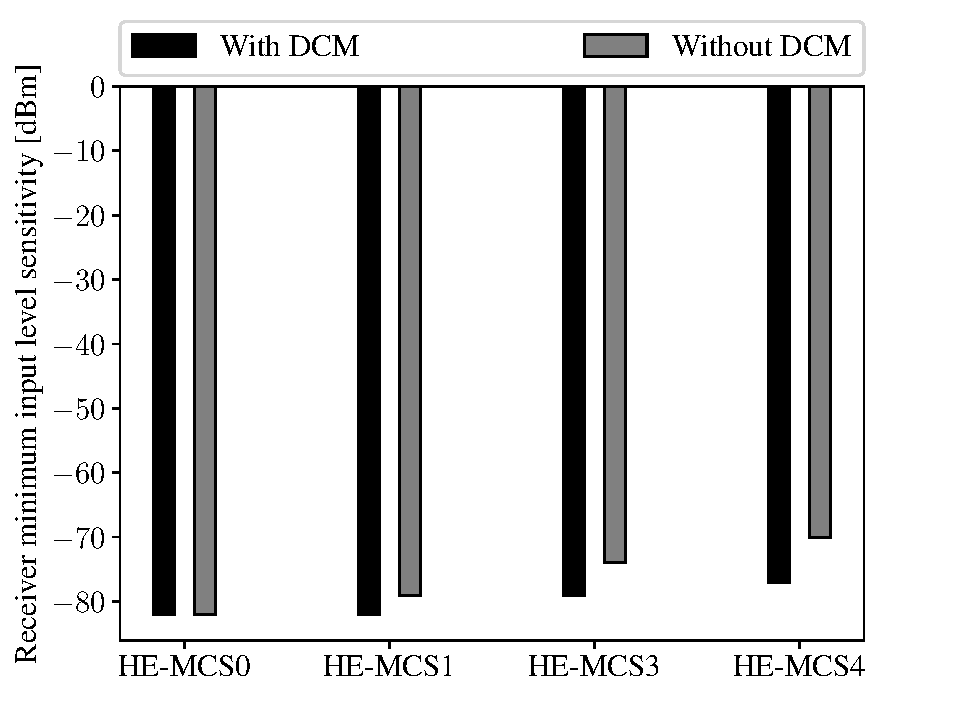
\includegraphics[width=0.75\textwidth]{figures/Receiver_minimum_DCM}
	\caption{Receiver minimum input level sensitivity for different HE-MCS values according to \cite{noauthor_ieee_2021}, where \ac{PER} is less than \SI{10}{\percent}}%
	\label{fig:ReceiverSensitivityDCM}%
\end{figure}

A similar development of the receiver minimum input sensitivity can also be observed for higher \ac{BW}, except
that the lowest value increases with \ac{BW}.

The higher probability of achieving data is reached at the expense of the data rate.
The same amount of data now takes twice as long to transmit.

\cite{noauthor_ieee_2021} lists the theoretically possible data rates.
These reveal that the maximum achievable data rate with DCM is only half of the attainable data rate without DCM.

Support for \ac{DCM} is only optional in the IEEE 802.11ax standard and can only be used for HE-\ac{MCS}-\num{0},
HE-\ac{MCS}-\num{1}, HE-\ac{MCS}-\num{3} and HE-\ac{MCS}-\num{4} for \numrange{1}{2} spatial
transmission streams \cite{noauthor_ieee_2021}.

\textcite{jacob_system-level_2020} and \textcite{triwinarko_phy_2021} mention plans,
to allow using \ac{DCM} in the physical layer of IEEE 802.11bd.

\begin{comment}
	Allowed relative constellation error versus constellation size RMS error over subcarriers and Frequency
	
	Table 27-51—Receiver minimum input level sensitivity
	
	Table 27-52—Minimum required adjacent and nonadjacent channel rejection levels
	optional feature \cite{noauthor_ieee_2021}
	
	\ac{HE} \ac{SU} \ac{PPDU} \ac{HE} \ac{ER} \ac{SU} \ac{PPDU} not for GI 800 ns \cite{noauthor_ieee_2021}
\end{comment}

\subsubsection*{\acf{ER}}
Since IEEE 802.11ax, the \ac{ER} Mode exists, which defines the new \ac{HE} \ac{ER} \ac{SU} \ac{PPDU} as physical layer amendment
\cite{noauthor_ieee_2021,afaqui_ieee_2017} .
\textcite{deng_ieee_2017} explains that the \ac{HE} \ac{ER} \ac{SU} \ac{PPDU} format is intended to extend the range of
a single station to access point transmission.
According to the authors, this is accomplished by the \ac{PPDU} containing a repetition of the HE-SIG-A field.

In addition, the authors explain that the preamble transmission power is boosted
to guarantee reliable transmission for longer ranges.
The power-boost is limited to additional \SI{3}{\decibel}
in \cite{noauthor_ieee_2021,jacob_system-level_2020}.

The IEEE 802.11ax \cite{noauthor_ieee_2021} standard defines that the \ac{HE} \ac{ER} \ac{SU} \ac{PPDU} format may only be used
when 20 Mhz transmissions with either 242-Resource Unit with HE-MCS-0 - HE-MCS-2 or 106-Resource Unit with HE-MCS-0 are used on a spatial stream.
In addition, one can use \ac{DCM}.
\textcite{sauter_wireless_2022} defines the Resource Unit as fragments of a Wi-Fi channel. The number before the Resource Unit
indicates the number of subcarriers which are part of the Resource Unit.

Optionally, the \ac{HE} \ac{ER} \ac{SU} \ac{PPDU} may also be transmitted with a \ac{GI} of \SI{800}{\nano\second},
where an additional application of \ac{DCM} is forbidden.

\textcite{jacob_system-level_2020} and \textcite{triwinarko_phy_2021} add that it is planned to use
the \ac{ER} mode also in the IEEE 802.11bd standard.

\subsubsection*{\acf{MIMO}}
In order to further exploit the physical layer capabilities, the single transmitting and receiving antenna systems called Single-Input-Single-Output can be extended to \ac{MIMO} - systems.
\textcite{sauter_wireless_2022} describe the idea behind \ac{MIMO} as the usage of multiple transmit antennas and multiple receiving antennas. Spatial multiplexing is used so that the transmitted signals
from each antenna are reflected differently on objects and can thus be received from different directions at the receiver antennas.

The authors explain that since IEEE 802.11n, it is possible to use up to \num{4} MIMO streams.
This number was increased again to up to \num{8} MIMO streams in IEEE 802.11ax \cite{noauthor_ieee_2021}.
Since data can be sent simultaneously via each MIMO stream,
the theoretical data rate can thus increase proportionally depending on the usable streams.
The mechanism is called \ac{SU}-\ac{MIMO} \cite{noauthor_ieee_2021}.

\textcite{sauter_wireless_2022} mentions that since IEEE 802.11ac it is possible to use Downlink \ac{MU}-\ac{MIMO},
which allows an \ac{AP} to transmit data to multiple \ac{STA} via different available \ac{MIMO} streams simultaneously.
According to the authors, \ac{MU}-\ac{MIMO} can increase the network throughput.
IEEE 802.11ax introduced \ac{MU}-\ac{MIMO} in the Uplink direction \cite{noauthor_ieee_2021}, where multiple \ac{STA} can transmit data simultaneously to the \ac{AP} via different available \ac{MIMO} streams.
MU-\ac{MIMO} DCM can also be applied in IEEE 802.11ax \cite{noauthor_ieee_2021}.

Another \ac{MIMO} technique is \ac{OFDMA}, which can be utilized since IEEE 802.11ax \cite{noauthor_ieee_2021, avallone_will_2021, omar_survey_2016}.
\textcite{avallone_will_2021} explains that \ac{OFDMA} enables an \ac{AP} to transmit data to multiple \ac{STA} simultaneously by dividing the available bandwidth into \ac{RU} and assigning each \ac{RU} to a \ac{STA}.
The authors add that \ac{OFDMA} can be used in both the uplink and downlink direction.
The \ac{AP} can choose the best suited \ac{RU} for each \ac{STA} and thus increase the Signal-to-Interference-plus-Noise Ratio \cite{khorov_tutorial_2019}
\textcite{behara_performance_2022} adds that \ac{OFDMA} is designed to improve the per-user throughput in high-density networks, e.q.
stadiums, airports or public transportation systems.

\subsubsection*{\acf{STBC}}
\textcite{abbas_efficient_2016} further explains that \ac{MIMO} spatial streams can be utilized to enhance the
quality of the received signal.
The Technology is called \ac{STBC}.
\textcite{santumon_space-time_2012} explains as follows.
\ac{STBC} is a technique used in Wi-Fi networks to improve the reliability and robustness of wireless communications.
\ac{STBC} encodes multiple redundant copies of data at the transmit side, which are transmitted in different spatial streams to
reduce fading and interference effects.
At the receiver side, these multiple copies are combined using a maximum likelihood detector
to retain a high-quality signal and decrease the \ac{PER}.


Here, \textcite{stamoulis_impact_2003} has investigated the potential effect of \ac{STBC} on Wi-Fi.
Their simulations showed that \ac{STBC} increase the range and robustness for IEEE 802.11a.
In addition, the authors concluded that \ac{STBC} increases the \ac{SNR} in nearly all cases at the same throughput or
even allows higher \ac{MCS} values to be used,
thus allowing a higher throughput at the same \ac{SNR}.
This results in \ac{STBC} improving the reliability and robustness of wireless communications.

\textcite{ghosh_error_2014} analyzed the error rate performance for an increased number of used antennae and found
that a lower bit error rate can be achieved
when increasing the number of transmit antennas with \ac{STBC}.

\textcite{gast_80211n_2012} and \textcite{sauter_wireless_2022} mention that \ac{STBC} can extend the signal range
due to the increased robustness.


IEEE 802.11ax stations can optionally use \ac{STBC} the following conditions \cite{noauthor_ieee_2021}:
\begin{itemize}
	\item DCM is not applied
	\item The number of spatial streams is \num{2}
	\item The \ac{GI} is not \SI{0.8}{\nano\second} and the symbol length is not \SI{12.8}{\micro\second}
\end{itemize}

\textcite{gast_80211n_2012} states that \ac{STBC} is only supported in \nicefrac{1}{5} of the Wi-Fi-certified devices.



\begin{comment}
In addition to the physical layer parameters already discussed, other technologies can be applied. IEEE 802.11ax
Beamforming
OFDMA
Group addressed frames
HE Capabilities nur so gut, wie das schlechteste Glied
\end{comment}






The next layer in the OSI model is the Data Link Layer.
The Data Link Layer consists of Medium Access - and Logic Link Control functionalities.


According to \textcite{kauffels_wireless_2002}, the medium access control functionalities cover network entry - ,network authentication - and media access methods.
The author explains, that every \ac{AP} send beacon frames periodically to synchronise its stations in the \ac{BSS} and that the beacon frame contains the \ac{SSID}, which identifies the \ac{BSS} or \ac{ESS} of the station. \textcite{sauter_wireless_2022} adds that a beacon frame contains a \SI{16}{\bit} - long capability information element. Each bit here signals that the \ac{AP} provides a particular function or has a specific feature. 

\textcite{kauffels_wireless_2002} explains the procedure for network entry of a station. A station can use the passive or the active scanning mode. In passive scanning mode, the station listens for a beacon frame in the various transmission channels. Alternatively, in active scanning mode, a station can also send out a probe frame. This can contain an already known \ac{SSID} to test the presence of the \ac{AP}. To get an \ac{AP} in range, the probe-frame can also contain a broadcast SSID that causes all nearby \ac{AP}s to respond. The response of an \ac{AP} to the probe frame is the probe-response frame, which contains the same information as a beacon frame. With the information from the beacon frame, a station can start the authentication process.
 
For this process, \textcite{kauffels_wireless_2002} names the two methods Open System Authentication and Shared Key Authentication. \textcite{sauter_wireless_2022} explains that Open System Authentication is based on a device making an authentication request to the \ac{AP}. If the \ac{AP} answers with a positive status in the Authentication Frame, the station is included in the \ac{BSS}. The actual encryption and authentication is then performed by the \ac{WPA} functions. The author points out that Shared Key Authentication is no longer used today. 

 the IEEE 802.11 standard describes the two media access methods \ac{DCF} and \ac{PCF}.

\textcite{sauter_wireless_2022} explains that \ac{DCF} is based on the media access method \ac{CSMACA}. In \ac{CSMACA} a device that is willing to transmit senses in the air transmission medium for a transmitting activity. If no other device is transmitting, the device can transmit. In the case of transmit activity, the terminal must wait at least until the transmission and \ac{DIFS} are over.
Since data transmission via the air transmission medium is very vulnerable to errors, the standard IEEE 802.11 requires that each received packet must be confirmed with an \ac{ACK} frame.
The \ac{DIFS} ensures that an \ac{ACK} frame can be sent before another station uses the same channel to send a data frame. 
To avoid multiple devices transmitting at the same time after \ac{DIFS}, each ready-to-transmit device determines a random backoff time. The device with the shortest backoff time transmits next and all other ready-to-transmit devices restart the media access procedure. In case two devices start sending next because they both randomly chose the shortest backoff time, the transmitted signal will interfere and the packets will not be answered with an \ac{ACK} frame.
In case of such a faulty transmission, the backoff time of the ready-to-transmit devices can increase exponentially afterwards.

To share the knowledge of a transmission time and the subsequently interframe space, a packet contains a \ac{NAV} that specifies the time the air transmission medium is used.

In various network architectures the "hidden station"-problem may occur. As you can see in \autoref{fig:hidden_station}, Station A is not able to sense a transmission of station B and vise versa. In case of simultaneous transmission of both stations, interference around the \ac{AP} may occur. 
\begin{figure}%
	\centering
	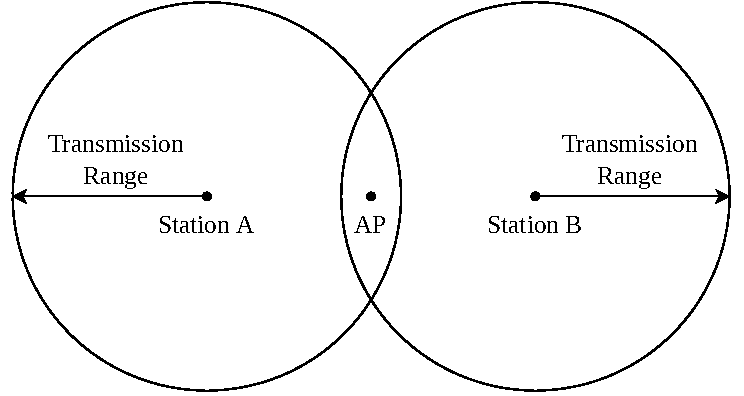
\includegraphics[width=0.75\textwidth]{figures/hidden_station.pdf}
	\caption{Hidden Station Problem}%
	\label{fig:hidden_station}%
\end{figure}


Um das hidden station problem zu umgehen kann eine Station nach \textcite{sauter_wireless_2022} 
Point coordinator 
ohne Wettbewerb mit optionaler Priorisierung

PIFS interval kürzer, 
beacon frame
CF Parameter set-element
\todo{nicht genauer eingehen, weil nicht relevant für die Arbeit? Darf ich das schreiben?}

CSMA /CA
Point Coordination Function

\textcite{sauter_wireless_2022}
DCF oberbegriff für CSMA /CA
 
 
Short Interframe Space SIFS ACK Frame 
 
Hidden Station Problem 
CTS and RTS
 
IEEE 802.11e DCF erweiterung für Video Streaming

CSMA CA Backoff zeit
Network allocation Vector NAV Zeitspanne Datensendungsdauer

MAC Header

Netzeintritt:
passives und Aktives Scanning
Service Set Identifier
Timing Synchronisationsfunktion TSF Timer-Wert

\textcite{sauter_wireless_2022}
every package management or usage data send ackknowledgement

Hidden Station Szenario
Reservieren
RTS CTS
meist nicht konfiguriert / ausgeschalten, bei großen Paketen sinnvoll



Authentifizierung
- Open System -Authentification
- Shared key Authentification
(nach neu nicht mehr verwendet


\subsection{IEEE 802.11ac - Wi-Fi 5}
The 5th generation WLAN is \ac{ac} and operates in the \SI{5}{\giga\hertz}  frequency range \cite{dhawankar_throughput_2018}.

According to \textcite{perahia_gigabit_2011}, \ac{ac} is a further evolution of IEEE 802.11n, where \ac{ac} adds to the known bandwidth of \text{IEEE 802.11n} of \SI{40}{\mega\hertz} the bandwidths \SI{80}{\mega\hertz},\SI{160}{\mega\hertz} and the interrupted bandwidth of \SI{80}{\mega\hertz} + \SI{80}{\mega\hertz}.

nach \textcite{sauter_wireless_2022} ist die Aufspaltung in zwei 80 Mhz Kanäle sehr nützlich, wenn das frequenzband reservierte Regionen enthält. Dadurch kann ein 160 Mhz breiter Kanal um  eine reservierte region des frequenzbandes gebaut werden.

The modulation technique used is \ac{OFDM}.
Additionally, a new \ac{MIMO} Downlink functionality for multiple users, called DL MU-MIMO, with up to 8 partial streams is introduced according to the authors. Together with the new \ac{MCS} from 64 \ac{QAM} to 256 \ac{QAM}, these three enhancements ensure that a higher data rate can be achieved. The maximum data rate is \SI{6.9}{\giga\hertz} according to the authors.

As declared by \textcite{abdelrahman_comparison_2015}, the 5th generation of WLAN has made it possible to expect better performance as in addition to a longer communication range compared to the previous IEEE 802.11 standards This statement could be proven at least for indoor range.  \textcite{dhawankar_throughput_2018} were able to demonstrate that \ac{ac} with a range of over \SI{60}{\metre} enables a longer indoor communication range than previous IEEE 802.11 standards.


new Physical Layer Very High Throughput (VHT) Physical Layer

80 Mhz

Beamforming 

\subsection{IEEE 802.11ax - Wi-Fi 6}

The 6th generation of WLAN is \ac{ax}. \textcite{khorov_tutorial_2019} reveals what has changed from \ac{ac} to \ac{ax}. For this, the authors make the following statements.

\ac{ax} uses the same bandwidths in the \SI{5}{\giga\hertz} range and can also operate in the \SI{2.4}{\giga\hertz} frequency range with a maximum bandwidth of \SI{40}{\mega\hertz}. Similar to DL MU transmission, \ac{ax} enables UL MU transmissions. These can also use \ac{OFDMA} in addition to the already known \ac{MIMO} of \ac{ac}. \ac{OFDMA} groups the orthogonal frequency subcarriers into \ac{RU}s, which can be selected by the transmitter for optimal transmission to the receiver. This increases the \ac{SINR}.

An extension in the PHY layer are the new \ac{MCS}'s of up to 1024-\ac{QAM}. However, these should only be used with very good channel characteristics.
 For better outdoor communication \ac{ax} increases the \ac{OFDM} symbol duration from \SI{3.2}{\micro\second} for \ac{ac} to up to \SI{12.8}{\micro\second} and the \ac{OFDM} Guard Interval from a maximum of \SI{0.8}{\micro\second} for \ac{ac} to up to \SI{3.2}{\micro\second}.   
 
MIMO und OFDMA MU Streams

BSS Coloring

Backward Kompatibilität über CTS Reservierungen.

Tabelle Vergleich

\begin{table}
	\centering
	\begin{tabular}{>{\raggedright}p{1.7cm}p{5.4cm}p{3.4cm}}
		\toprule
		Parameter & IEEE 802.11ac & IEEE 802.11ax \\
		\midrule
		Frequency bands & \SI{5}{\giga\hertz}&
		\SI{2.4}{\giga\hertz}, \SI{5}{\giga\hertz}, \SI{6}{\giga\hertz}\\
		Symbol Length & \SI{3.2}{\micro\second}&
		\SI{12.8}{\micro\second}\\
		\ac{OFDM} Subcarrier Spacing &
		\SI{312.5}{\kilo\hertz} &
		\SI{78.125}{\kilo\hertz} \\
		\ac{OFDM} Subcarriers in \SI{80}{\mega\hertz} &
		256 &
		1024 \\
		max. \ac{MCS} &
		256 -\ac{QAM} &
		1024 -\ac{QAM} \\
		max. \ac{GI} &
		\SI{0.8}{\micro\second} &
		\SI{3.2}{\micro\second} \\
		\bottomrule
	\end{tabular}
	\caption{Comparison of IEEE 802.11ac and IEEE 802.11ax}
	\label{tab:SensorNetworkApplications}
\end{table}

\iffalse
\section{Modell für drahtlose Übertragungssysteme}

Abb 2.3.1  Modell einen Übertragungssystems

Beschränkungen und Regelungen Frequenzwahl, Sendeleistung

Analoger Kanal Störungen: thermisches Rauschen, Nebensprechen, Impulsstörungen
\fi

\section{Harvest and Loading Processes as a Use Cases for \ac{WIC}}
The Forage harvester has proven to be an essential agricultural machine for harvest
ing and loading forage. \textcite{seifert_feldhacksler_1962} define a forage harvester
as an agricultural loading machine for nearly all types of animal feed. According to the authors, a  forage harvester can load the following animal feed by mounting different cutting and loading devices: Hey, Straw, Corn, Grass and Clover.
\begin{figure}%
	\centering
	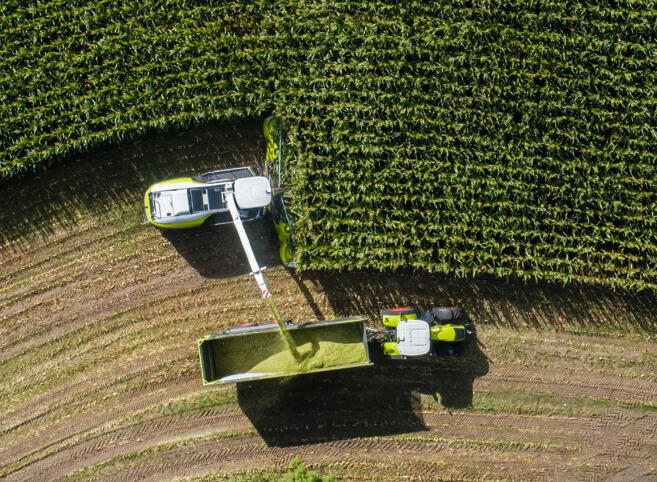
\includegraphics[width=0.6\textwidth]{figures/claas_harvest_side.png}
	\caption{\ac{FH} and \ac{TM} while }%
	\label{fig:normal}%
\end{figure}

In the harvesting and loading process, a \ac{TM} typically drives alongside or behind the \ac{FH} so that the \ac{FH} can load the harvested goods onto the trailer of the \ac{TM} using the spout. Drivers operate both machines and try to keep the speed and distance so that the spout only throws the harvested goods into the trailer of the TM. An image of a corn harvesting and loading process can be seen in \autoref{fig:normal}.

Taking a corn harvest scenario as an example, I looked up key figures in \cite{faustzahlen2018}, a standard reference book in agricultural literature. This book contains key figures of agricultural processes, which 80 experts have compiled. The key figures, which are shown in \autoref{tab:DataSilageHarvest}, are dependent on the \ac{PPD} and show the large amount of forage harvested by a  \ac{FH} every hour.
\begin{table}[H]
	\centering
	\begin{tabular}{>{\raggedright}p{4.9cm}p{1.8cm}p{1.8cm}p{1.8cm}}
		\toprule
  		\ac{PPD} &  \SI{20}{\tonne\per\hectare} & \SI{30}{\tonne\per\hectare} & \SI{50}{\tonne\per\hectare}\\
		\midrule
		Required \ac{TM}s & \num{5}&
		\num{7} & \num{10} \\
		Harvested volume in \si{\cubic\metre\per\hour} &
		\num{285.7}-\num{333.3}
		& \num{428.6}-\num{500.0} &
		\num{595.7}-\num{695.0}\\
		Filled \ac{TM} loads in \si{\per\hour} &
		\num{5.7} - \num{6.7}
		& \num{8.6} - \num{10.0} &
		\num{11.9} - \num{13.9}\\
		Harvested mass in \si{\tonne\per\hour} & \num{100}
		& \num{150} &
		\num{208.5} \\
		\bottomrule
	\end{tabular}
	\caption{Key figures from \cite{faustzahlen2018} of corn harvest of a \ac{FH} with a working width of \SI{6.2}{\metre} in a \SI{80}{\hectare}-field in regards to \ac{PPD}}
	\label{tab:DataSilageHarvest}
\end{table}

The harvesting and loading processes are examples of the use of agricultural Platooning Services as described by 
\textcite{zhang_method_2009}.
This Platooning Service creates a leader and follower system where an uncrewed agricultural machine follows a leading operated agricultural machine.
The operated \ac{FH}, as a leader, sets the path and speed and transmits the data via \ac{WIC} to the \ac{TM}. Based on the path and speed data of the \ac{FH}, \ac{TM} follows unmanned with a longitudinal and lateral offset, as \autoref{fig:offset} displays.
\begin{figure}[H]
	\centering
	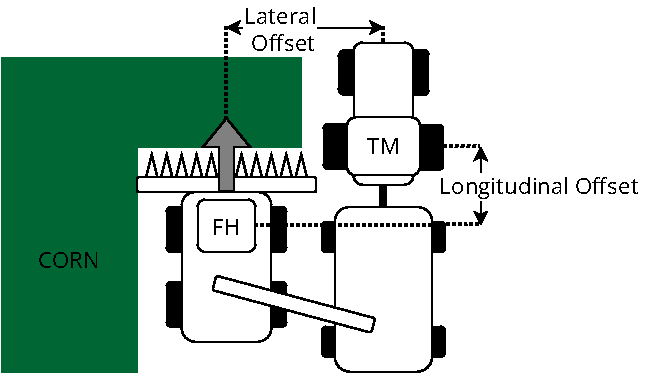
\includegraphics[width=0.65\textwidth]{figures/offset_platoon.pdf}
	\caption{Lateral and longitudinal Offset between the two agricultural machines \ac{FH} and \ac{TM} in a corn harvest scenario}%
	\label{fig:offset}%
\end{figure}

The application of platooning services offers many advantages.
The \ac{TM} is positioned optimally to the \ac{FH} so that the forage can be loaded ideally from the \ac{FH} onto the \ac{TM}.

Because, as displayed in \autoref{fig:workforce_agri}, fewer and fewer workers are working in agriculture, platooning services for harvest and loading processes can save and free up labour for other activities \cite{liu_automation_2022}. As stated in \autoref{tab:DataSilageHarvest}, already ten drivers for the \ac{TM}s are needed in the corn harvest process with a high \ac{PPD}. Using an agricultural Platooning Service, each \ac{TM} can drive unmanned in the field, leading to fewer workers needed in the corn harvest process.

\begin{figure}[H]
	\centering
	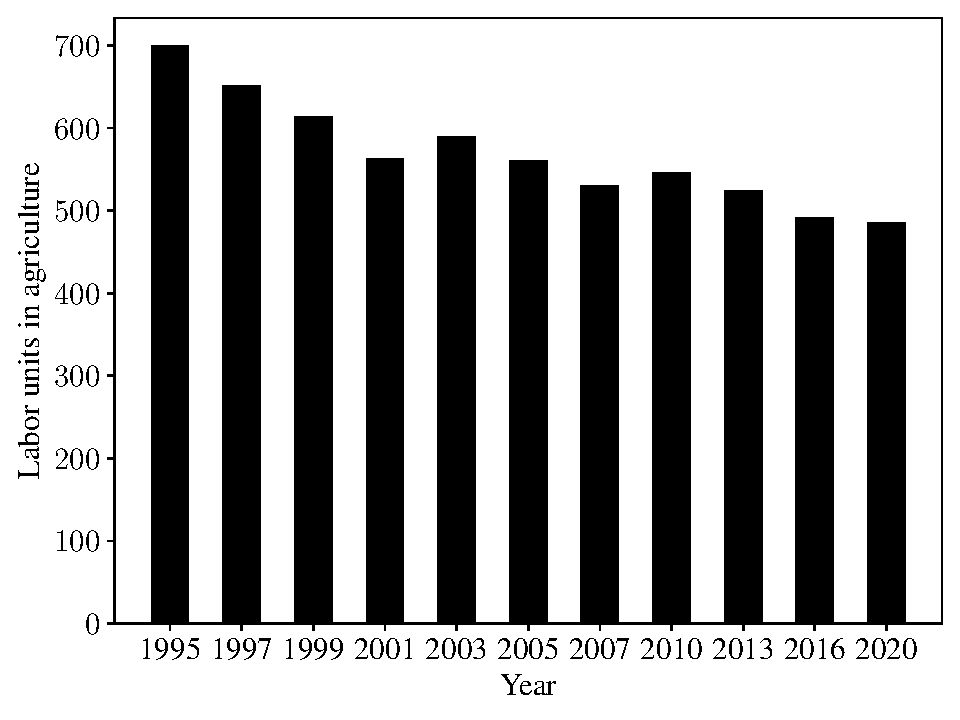
\includegraphics[width=0.75\textwidth]{figures/WorkForceAgriculture.pdf}
	\caption{Decrease in the agricultural labor force in Germany based on the data from \cite{bmel2020}}%
	\label{fig:workforce_agri}%
\end{figure}

\textcite{smolnik_5g_2020} adds that platooning services at the platoon level can reduce drivers' workload so that they can focus on optimally adjusting the machines.
In addition, \ac{TM}s can be guided to the \ac{FH}s in a targeted manner so that logistics processes in the field can be improved.

At the same time, the harvest and loading processes are examples of the video streaming \ac{WIC} use case. During these harvest and loading processes, the spout of the \ac{FH} must be controlled to set the loading position of the forage into the trailer of the \ac{TM}.

According to \textcite{murcia_quadrotor_2014}, different spout guidance and control systems have been developed to automate the filling of the trailer. Spout guidance and control systems use a camera attached to the spout to determine the fill volume at each point of the trailer via machine vision and set the spout to fill the empty parts accordingly. The author describes Autofill - systems from Claas and Intellifill - systems from CNH Industrial as examples of spout guidance systems. 

Streaming the video of a camera at the spout from the \ac{FH} to the \ac{TM} would be a practical application of the video streaming use case in the harvesting process. If the \ac{TM} driver can watch a live stream of the trailer's fill level, he will always be
informed and knows when the trailer is full and can drive the forage back to the
farm.

\chapter{Analyzing Corn Harvest Process Data}

To gain a better insight into requirements of the \ac{WIC} use cases Platooning and Streaming Services, I analysed process data of a corn harvest scenario as the example for I collected GPS tracks of  a  \ac{FH} and two to three \ac{TM}s harvesting corn on a field in Germany on two days in September. For this, I placed tablets in the driver's cabs of  a  \ac{FH} and three \ac{TM}s, which recorded the position and speed in an NMEA data stream of the tablet's GPS every second. 

% wahrscheinlich raus
The workflow for collecting the corn harvest process data was as follows. 
I handed out the tablets to the drivers, which left the farm with the tablets in the driver's cabs to drive to the field in the morning. The tablets recorded the position and speed of the \ac{FH} and the \ac{TM}s all day. During breaks, the tablets continued to capture the NMEA data stream of their GPS even if the positions and speed did not change.

After recording the process data, I anonymized it. 
First, I deleted data points of the log files until the recorded accuracy of the following data points was less than \SI{2}{\metre}. Then, I replaced the timestamp and the date for all data points with a continuous index.

To gain a better insight into requirements of the \ac{WIC} use cases Platooning and Streaming Services, I analysed process data of a corn harvest scenario as the example for I collected GPS tracks of a  \ac{FH} and two to three \ac{TM}s harvesting corn on a field in Germany on two days in September. For this, I placed tablets in the driver's cabs of a  \ac{FH} and three \ac{TM}s in the morning, which recorded the position and speed in an NMEA data stream of the tablet's GPS every time second. 

After I collected the tablets in the evening, I anonymised the recorded process data. 
Starting, I deleted data points of the log files until the recorded accuracy of the following data points was less than \SI{2}{\metre}. Then, I replaced the timestamp and the date for all data points with a continuous index.

After that, I anonymised the location data by adding a random offset to the GPS coordinates. As a result, this procedure moved the areas to a random location in the world with a continuous index as a timestamp, where the exact date is unknown.

The goal of analysing the corn harvest data was to investigate the machines moving in the working scenarios relative to each other. The machines' speed and distance in tracked harvest platoons data may result in new use case requirements, e.g. latency or communication range of Platooning and Streaming Services. The machinery movement profile can be used to identify when shadowing effects may occur in the work scenario or when machines meet in the field.

For this purpose, I built a dashboard with the Python framework \textit{Dash}\footnote{https://dash.plotly.com/introduction Accessed: 5.12.2022}. I initially plotted all the positions in a polyline for each machine
on a map in the dashboard. An added slider allows one to set a time interval that narrows down the data points for display in the dashboard. In addition, one could select which \ac{TM}s are displayed next to the \ac{FH}. For the chosen time interval, the distance and velocity difference between the selected \ac{TM}s and the \ac{FH} were plotted in graphs as time histories.

In the dashboard, I could get an overview of the machine's behaviour 
before, during, and after the overloading scenario.
The overview shows that a \ac{FH} is nearly always in the overloading process with a \ac{TM}. In doing so, the \ac{FH} may occasionally stay in the same place if the cutter is clogged or there is a transition of \ac{TM}s where a full \ac{TM} moves away from the \ac{FH} and an empty \ac{TM} catches up to the \ac{FH} to take over the forage.

A \ac{TM} is in a platoon with a  \ac{FH} if it is close to the \ac{FH} and they are moving at nearly the same speed. The distance between \ac{TM} and \ac{FH} increases during a turning manoeuvre on the field. Since both machines have different curve radii in a turning manoeuvre, a different machine's speed can be observed to finish turning simultaneously.
\textcite{smolnik_5g_2020} also describes these observations and indicates that this different speed adds a new level of complexity.

A new harvesting process begins as soon as the machines finish turning and are at the beginning of a new lane.
Again, the machines drive closely and nearly at the same speed to harvest and overload forage.

Furthermore, another \ac{TM} can sometimes be close to the \ac{FH}. This \ac{TM} is empty and waits to work with the \ac{FH} in the next platoon. For that purpose, the empty \ac{TM} drives close behind the current platoon at the same speed to not catch up even closer to the platoon and be ready in the vicinity.

Based on the above observations, I developed an intelligent algorithm for detecting platooning scenarios in the recorded harvest process data. It uses a weighted sum of distance and speed difference between \ac{FH} and \ac{TM} to detect the platooning scenarios.

For verification purposes, I displayed the found platoons scenarios on the map and confirmed the algorithm's functioning. 

Additionally, I implemented the following further verification method. 
I observed that a fully loaded \ac{TM} leaves the field via one of the field exits to bring the crop to a farm building. Via a check, if a \ac{TM} has left the field and thereby passed the exit after leaving a platoon, wrongly recognized platoons can be discarded.

\begin{figure}%
	\centering
	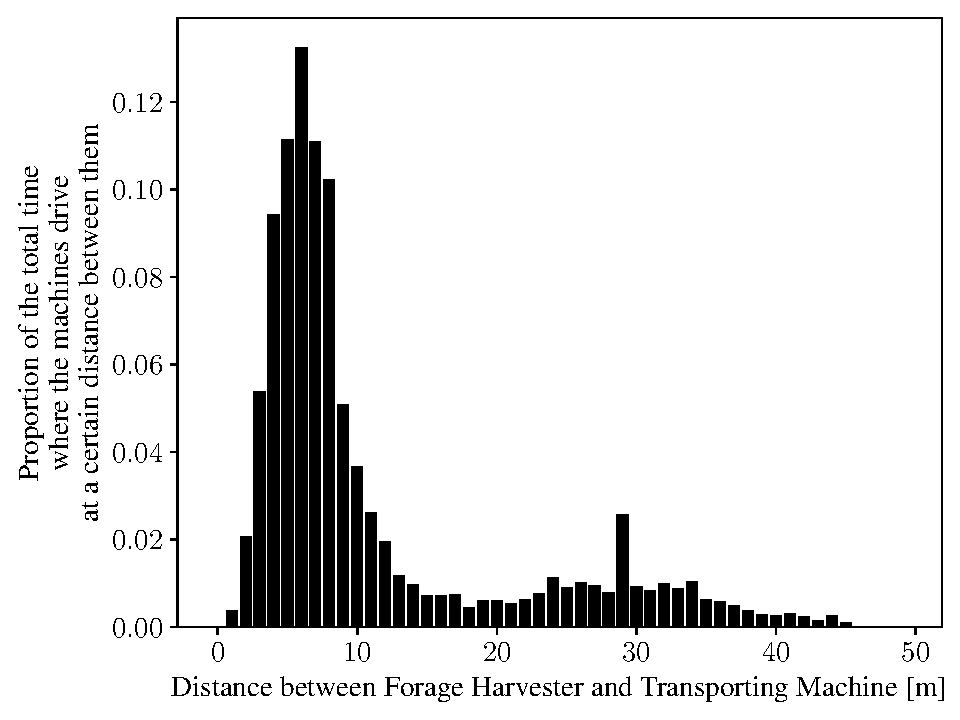
\includegraphics[width=0.85\textwidth]{figures/distanceHarvestSzenario.pdf}
	\caption{Distribution of time proportions where a given distance was between \ac{FH} and \ac{TM} in a harvest platoon scenario.}%
	\label{fig:distance}%
\end{figure}
\begin{figure}%
	\centering
	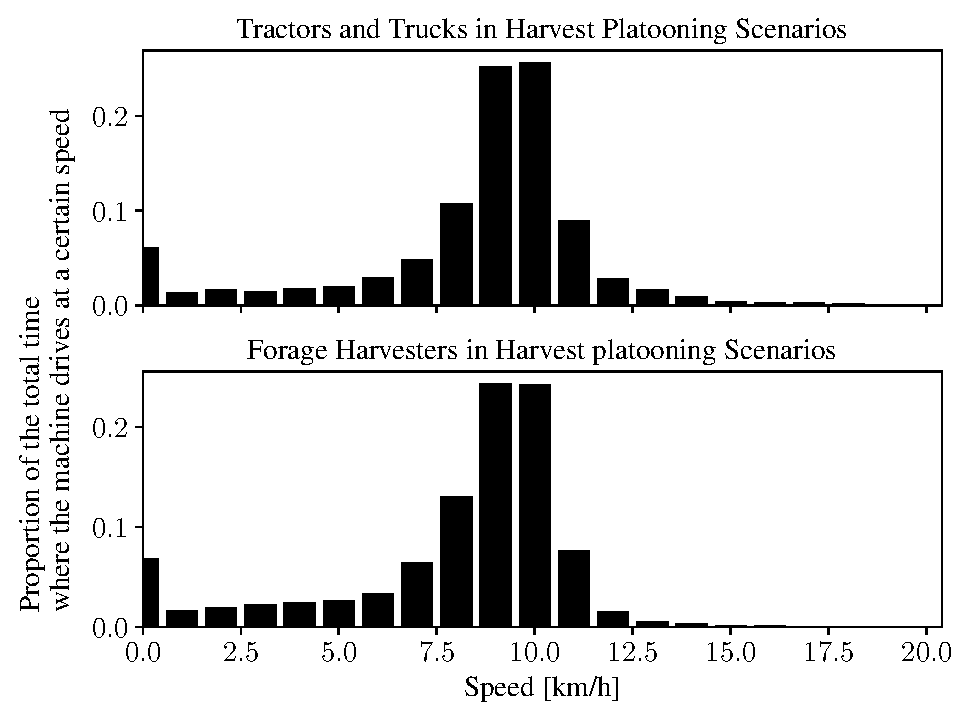
\includegraphics[width=0.85\textwidth]{figures/speedHarvestSzenario.pdf}
	\caption{Distribution of time proportions where \ac{FH} and \ac{TM} drove with a certain speed in a harvest platoon scenario}%
	\label{fig:speed}%
\end{figure}

After the platoons scenarios were correctly detected, I included the data points before each platoons scenario till a maximum distance of \SI{50}{\metre} between \ac{FH} and \ac{TM} was exceeded. These data points are also relevant to the requirements because at the beginning of an agricultural platooning service, the \ac{FH}, as the system leader, must be able to guide an empty \ac{TM} to the appropriate position for overloading.

For the detected data points of the platooning services from recorded data of the corn harvest, the proportion where the \ac{FH} and \ac{TM} move in a specific distance is shown in \autoref{fig:distance}. For the same data points, the proportion in which \ac{FH} and \ac{TM} move at a given speed is available in \autoref{fig:speed}.

These analysing results show that the \ac{TM} and the \ac{FH} usually move with a distance of less than \SI{10}{\metre}. In addition, the distance can also be higher, e.g. in turning manoeuvres or before the overloading process.

\textcite{smolnik_5g_2020} specifies the required communication range of platooning services in the corn harvest process as less than \SI{30}{\metre}.

One notable observation in \autoref{fig:speed} is that the \ac{FH} and \ac{TM}s in the corn harvesting platooning scenario often travel at a speed of approximately \SI{10}{\kilo\metre\per\hour}. This speed is significantly higher than the average speed of \SI{5.6}{\kilo\metre\per\hour} of a \ac{FH} in an entire corn harvesting process from \cite{faustzahlen2018}. It is necessary to classify that in the year of the recorded data was little precipitation, so the corn was not dense and high, and the last speed value is an average value of the entire corn harvest process, which can be calculated from the data in \cite{faustzahlen2018}.
Nevertheless, the recorded data shows that a platooning service in agriculture must also be designed for higher speeds. 

In \autoref{fig:speed} is a local maximum at a speed of \SI{0}{\kilo\metre\per\hour}. In a harvest platoon scenario, \ac{FH} and \ac{TM} can stand still briefly when the cutting device is jammed.
The driver's specific actuation usually clears the forage jam of the cutting device so that the platoon can continue its work.

\textcite{smolnik_5g_2020} defines an average speed of \SI{4.5}{\kilo\metre\per\hour} for the development of platooning services in the corn harvesting process. Depending on the \ac{PPD}, the speed can vary from \SIrange{2}{6}{\kilo\metre\per\hour} according to the authors.
The authors do not give a basis for the figures. However, the report is from the agricultural machinery manufacturer Claas, which is a major producer of \ac{FH} worldwide and thus should have expertise in the topic.

\textcite{klingler_agriculture_2018} investigated the suitability of IEEE 802.11p for \ac{WIC}. The authors detected that shadowing effects occur in the harvest scenario. The authors explain the effect because another tractor or the spout of the \ac{FH} was in \ac{LOS}.
\begin{figure}%
	\centering
	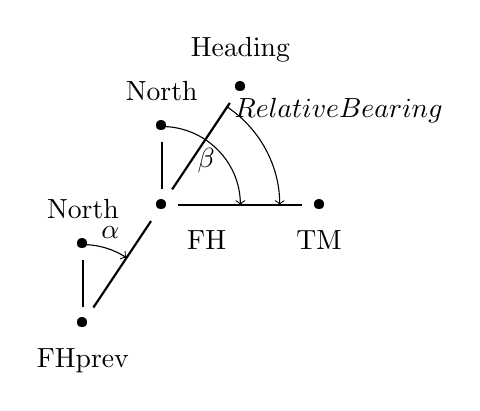
\begin{tikzpicture}
		\node[label=below right:FH](a) at (0,0) {\textbullet};
		\node[label=above:North](d) at (0,1) {\textbullet};
		\node[label=above:Heading](c) at (1,1.5) {\textbullet};
		\node[label=below:TM](b) at (2,0) {\textbullet};
		\node[label=below:FHprev](e) at (-1,-1.5) {\textbullet};
		\node[label=above:North](f) at (-1,-0.5) {\textbullet};
		\draw [thick] (a) -- (b);
		\draw [thick] (a) -- (c);
		\draw [thick] (a) -- (d);
		\draw [thick] (a) -- (e);
		\draw [thick] (e) -- (f);
		\draw 
		pic["$\beta$", draw, <-,angle eccentricity=0.8, angle radius=1.0cm]
		{angle=b--a--d}
		pic["$\alpha$", draw, <-,angle eccentricity=1.2, angle radius=1.0cm]
		{angle=a--e--f}
		pic["$Relative Bearing$", draw, <-, angle eccentricity=1.7, angle radius=1.5cm]
		{angle=b--a--c};
	\end{tikzpicture}
	\caption{Relative bearing between \ac{FH} and \ac{TM} which is calculated using the previous location of \ac{FH} by using $\beta$ and $\alpha$ for \autoref{eq:RelativeBearing}}%
	\label{fig:bearing_fh_tm}%
\end{figure}
I reviewed the recorded position data to get an overview of the \ac{TM}'s position relative to the \ac{FH}  in the overloading process. The relative bearing is the angle between B, and the heading of point A. Using the previous position of the \ac{FH}, the relative bearing between \ac{FH} and \ac{TM} can be calculated with the angles $\alpha$ and $\beta$ in \autoref{fig:bearing_fh_tm} as:
\begin{equation}\label{eq:RelativeBearing}
	Relative\_Bearing = \beta - \alpha	,
\end{equation}
Assuming that the \ac{FH} does not move backwards, the relative bearing describes the relative angle from the \ac{FH} to \ac{TM}. The result is displayed in \autoref{fig:bearing}. It can be observed that the \ac{TM} is mainly close to the \ac{FH} at an angle of \SIrange{30}{150}{\degree} at a distance between \SIrange{0}{10}{\metre}. 

\begin{figure}[H]
	\centering
	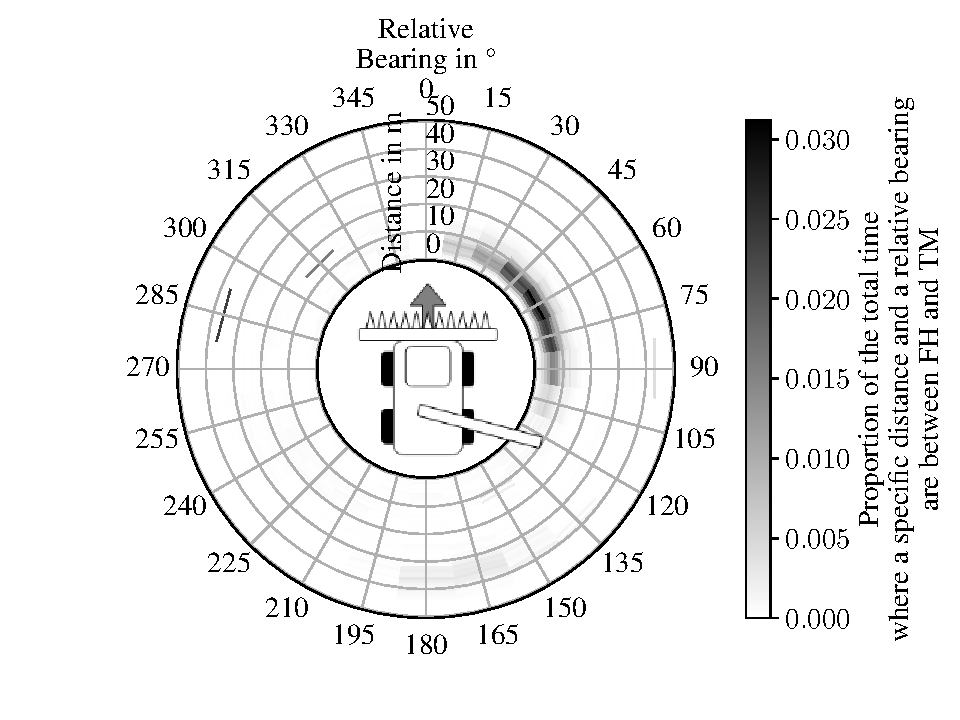
\includegraphics[width=0.99\textwidth]{figures/bearingHarvestScenario50.pdf}
	\caption{Distribution of time proportion at specific distances and relative bearings between \ac{FH} and \ac{TM}}%
	\label{fig:bearing}%
\end{figure}

In addition, it is noticeable that the machine can also be directly behind the \ac{FH}. This driving behind each other is common when a new part of the field is being cut in harvesting, as shown in \autoref{fig:startpart}. When there is a greater distance between \ac{TM} and \ac{FH}, the \ac{TM} is usually behind the FH at an angle of \SIrange{157.5}{187.5}{\degree}. At these moments, the \ac{TM} is empty and closes up to the \ac{FH} to operate in a new platooning Service together. 

\begin{figure}[H]%
	\centering
	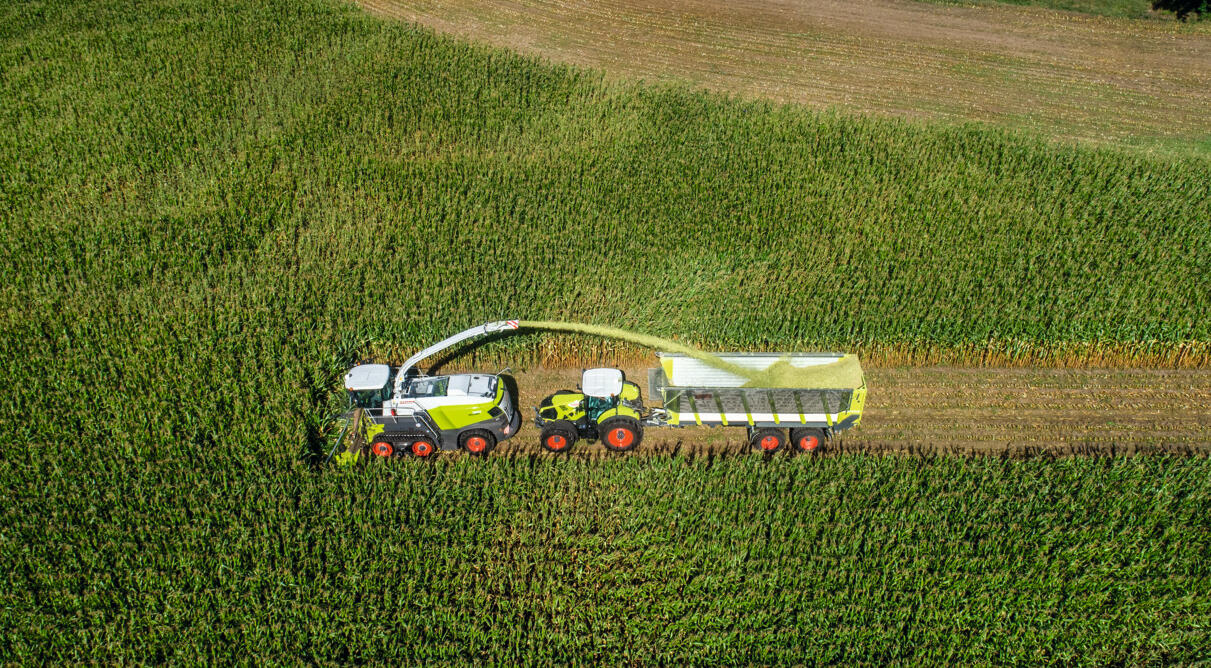
\includegraphics[width=0.8\textwidth]{figures/claas_harvest_behind.png}
	\caption{\ac{FH} and \ac{TM} start cutting a new field section}%
	\label{fig:startpart}%
\end{figure}

Another notable fact is that the \ac{TM} hardly ever stayed to the left of the \ac{FH}. Since the \ac{FH} often made left turns, the crop was usually already harvested to the right of the \ac{FH} so that the \ac{TM} could drive there without running over the crop. On rare occasions, the \ac{TM} was also to the left of the \ac{FH}. Such a platooning scenario can be an exception or a driving manoeuvrer to start cutting a new part of the field.   

The results reveal only a first impression of the harvest and loading process requirements. More data from around the world must be analyzed to make a general statement. The low rainfall this year has already resulted in a low plant population. This field condition made a higher process speed possible. To make a general statement, I should use data from different years because they can reveal different initial field conditions.


\TODO{
	Heading Annahme Vorwärts Fahrt. Ansonsten Überprüfen und nochmal Einzelfahrt plotten und anschauen. 
	Wie oft dreht sich das Heading ?
	Möglicherweise Rückwärtsfahrt erkennen? Oder WIC Requirements erwähnen? }


\chapter{Field Measurements}


\chapter{Developed architecture / System design / Implementation / ...}


\begin{itemize}
\item describe everything you yourself did (as opposed to the fundamentals chapter, which explains what you built on)
\item start with a theoretical approach
\item describe the developed system/algorithm/method from a high-level point of view
\item go ahead in presenting your developments in more detail
\item recommended length: approximately one third of the thesis.
\end{itemize}

\chapter{Simulation}
Seite 77 von 93 02 simulation.pdf
Propagation Model:
 Two Ray Ground only mathematics Rappaport
 Jakes Model
 Three Log Distance
 
 
 Data Simulation
 
 
 
\todo{QUESTIONS open 7 Möglichkeiten outdoor wifi
was für Effecte}

\todo{
Robustheit: Matlab? 
Goodput: ns3
Range: Matlab? Somehow? overview
other papers? 
Enough?
}
 
 
\section{ns-3 Network Simulator}

Bei der Wahl der Network Simulator Wifi 6 Implementierungen 


\todo{Warum nicht was anderes GNS3, MININET, ... ?}

According to \cite{ns3manual} ns-3 is a discrete-event network simulator project, which was founded in 2006. The ns-3 project is open source with a licence based on n GNU GPLv2 compatibility. It aims to procide an open, extensible network simulator for research and educational use. Ns-3 scripts can be written in C++ or Python.
ns-API Python uses models in C++
build system Cmake

ATM no pre-built libraries and packages for operating systems
 
The concept of ns3 is based on the abstraction of simulated systems. For this purpose, the term node was introduced for basic computing devices. The Node class offers the possibility to install protocol stacks and applications or to add peripheral cards and mobility models to the node.
Applications are the abstraction of the user-level applications, which represent an activity to be simulated. For this purpose, the applications use resources and functionalities provided by the system software of a node. An example for the 



\section{Data Rate}


\ac{GI} and \ac{CR}
\begin{figure}%
	\centering
	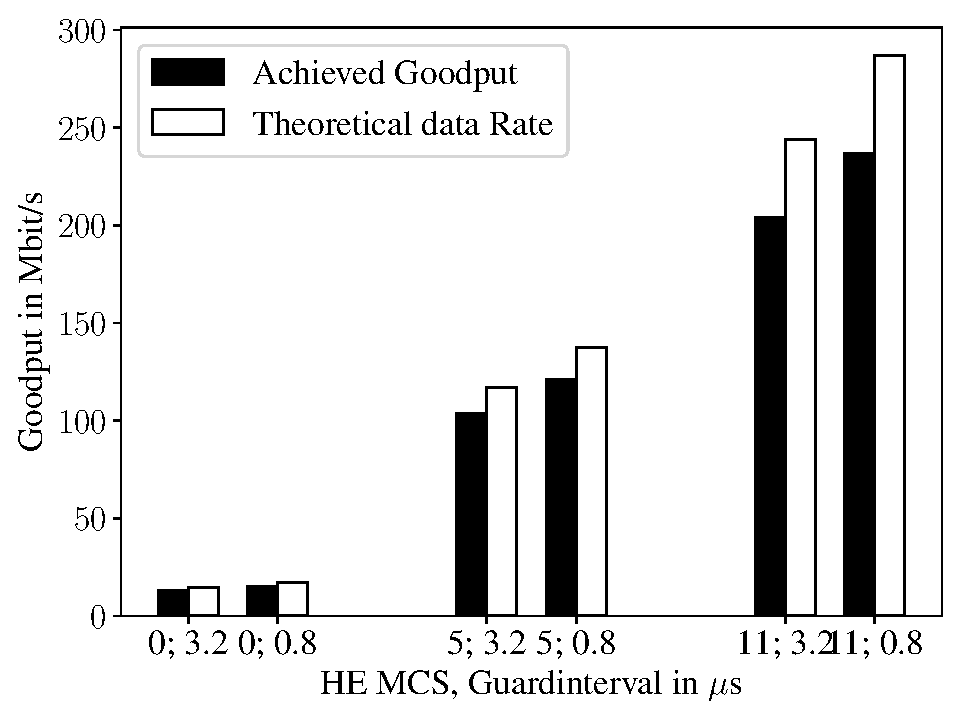
\includegraphics[width=0.95\textwidth]{figures/gi_dataRate_simulation.pdf}
	\caption{Achieved Goodput and theoretical Datarate of two WiFi 6 stations in Ad-Hoc Mode with \num{2} \ac{MIMO} streams and a bandwidth of \SI{80}{\mega\hertz} in regards to the number of \ac{MIMO} streams and the chosen \ac{MCS} and \ac{CR}}%
	\label{fig:Data_rate_GI}%
\end{figure}

atteninuation of bandwidth : 800ns : \SI{94}{\percent} \SI{89}{\percent} \SI{80}{\percent}

Factors apply for MCS0 but may also apply later

\begin{figure}%
	\centering
	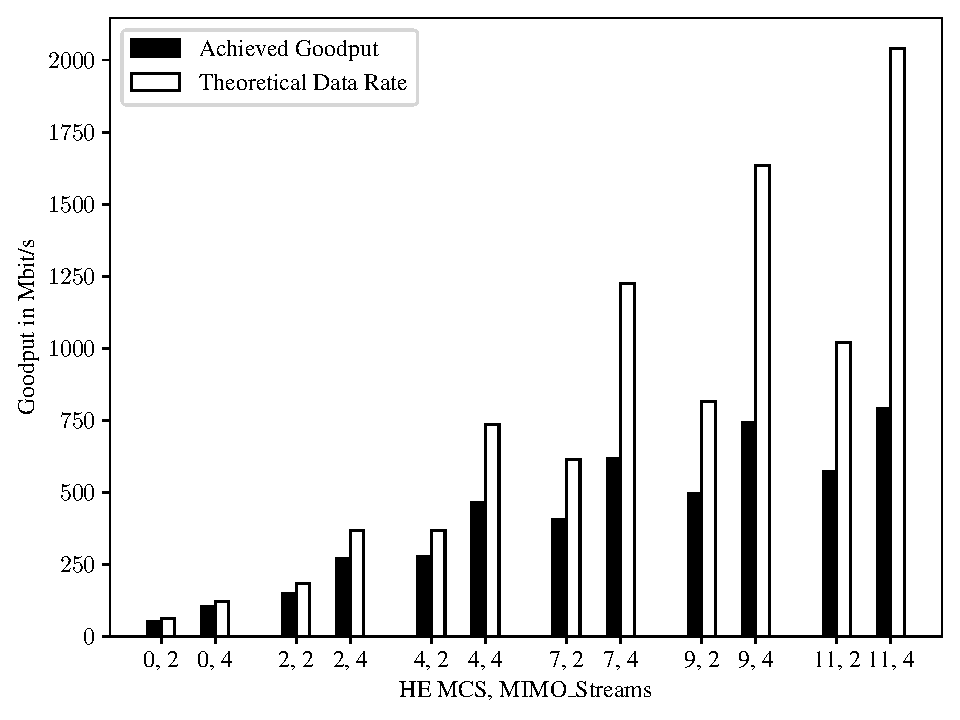
\includegraphics[width=0.95\textwidth]{figures/mimo_dataRate_simulation.pdf}
	\caption{Achieved Goodput and theoretical Datarate of two WiFi 6 stations in Ad-Hoc Mode with a \ac{GI} of \SI{3200}{\nano\second} and a bandwidth of \SI{80}{\mega\hertz} in regards to the number of \ac{MIMO} streams and the chosen \ac{MCS} and \ac{CR}}%
	\label{fig:Data_rate_Mimo}%
\end{figure}


\begin{figure}%
	\centering
	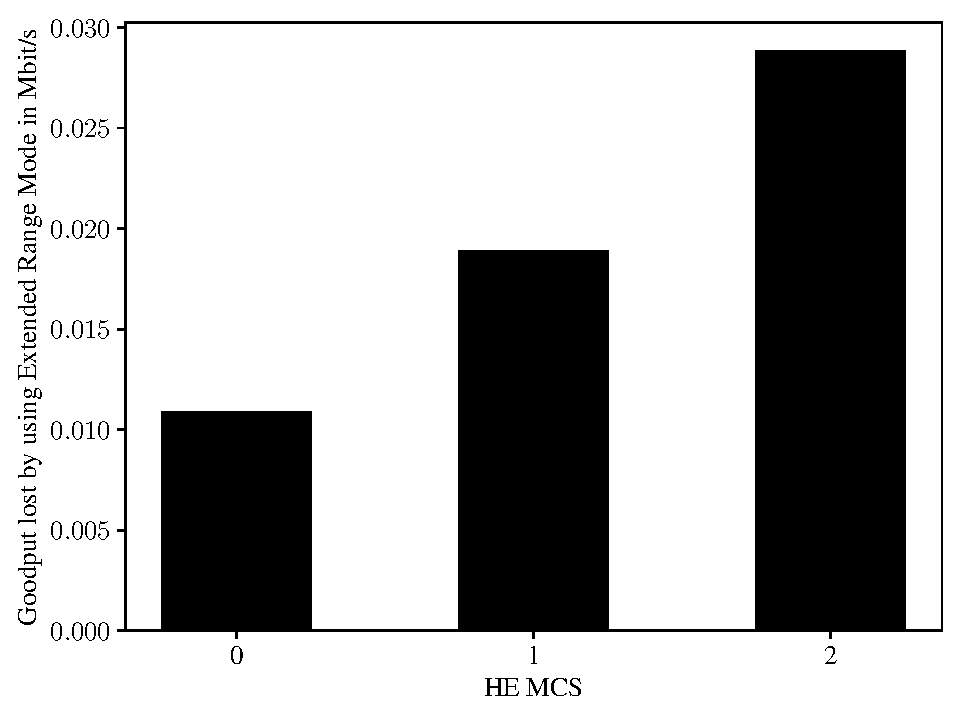
\includegraphics[width=0.95\textwidth]{figures/ER_dataRate_simulation.pdf}
	\caption{Achieved Goodput and theoretical Datarate of two WiFi 6 stations in Ad-Hoc Mode with a \ac{GI} of \SI{3200}{\nano\second} and a bandwidth of \SI{20}{\mega\hertz} in regards to the number of \ac{MIMO} streams and the chosen \ac{MCS} and \ac{CR}}%
	\label{fig:Data_rate_ER}%
\end{figure}

\todo{DataRate for STBC}
STBC and DCM * 2 payload / half data rate

\begin{figure}%
	\centering
	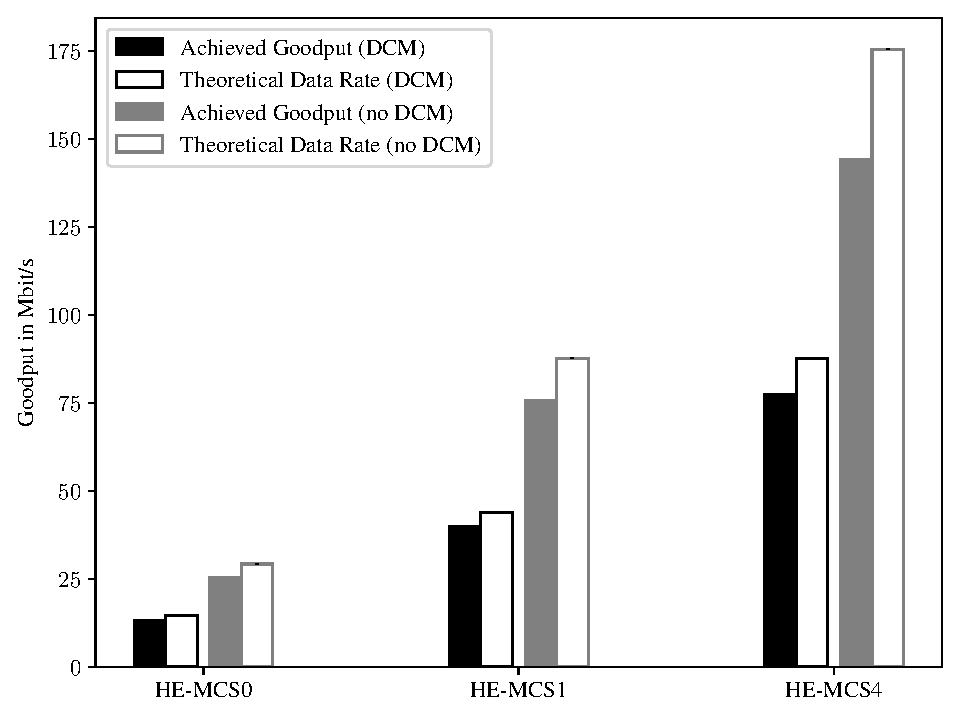
\includegraphics[width=0.95\textwidth]{figures/DCM_dataRate_simulation.pdf}
	\caption{Achieved Goodput and theoretical Datarate of two WiFi 6 stations in Ad-Hoc Mode with a \ac{GI} of \SI{3200}{\nano\second} and a bandwidth of \SI{40}{\mega\hertz} in regards to the number of the chosen \ac{MCS} and \ac{CR} and whether \ac{DCM} is enabled}%
	\label{fig:Data_rate_DCM}%
\end{figure}


But Latency? 
Robustness?

Fixed Wifi 6 devices: 4 Streams, 2.4, 5.0 Ghz
Fixed Wifi bd devices: 1 Stream, 5.9 Ghz, 

Leave it open for future work?
look for different chips?

Auf different paper stützen? 


\chapter{Evaluation}


\begin{itemize}
\item measurement setup / results / evaluation / discussion
\item whatever you have done, you must comment it, compare it to other systems, evaluate it
\item usually, adequate graphs help to show the benefits of your approach
\item each result/graph must not only be described, but also discussed (What's the reason for this peak? Why have you observed this effect? What does this tell about your architecture/system/implementation?)
\item recommended length: approximately one third of the thesis.
\end{itemize}



\chapter{Conclusion}


\begin{itemize}
\item summarize again what your paper did, but now emphasize more the results, and comparisons
\item write conclusions that can be drawn from the results found and the discussion presented in the paper
\item future work (be very brief, explain what, but not much how, do not speculate about results or impact)
\item recommended length: one page.
\end{itemize}

Untersuchen, welche Routing protocols

\cleardoublepage

\listofabbreviations
\clearpage

\listoffigures
\clearpage

\listoftables
\clearpage

\printbibliography

\end{document}
